\begin{figure}
%	\includegraphics[trim={0 15 0 0},clip,width=\linewidth]{vect/mod_ex}	
	\center
	\begin{minipage}{0.15\linewidth}
		\center\scriptsize
		Images
	\end{minipage}\hfill
	\begin{minipage}{0.84\linewidth}
	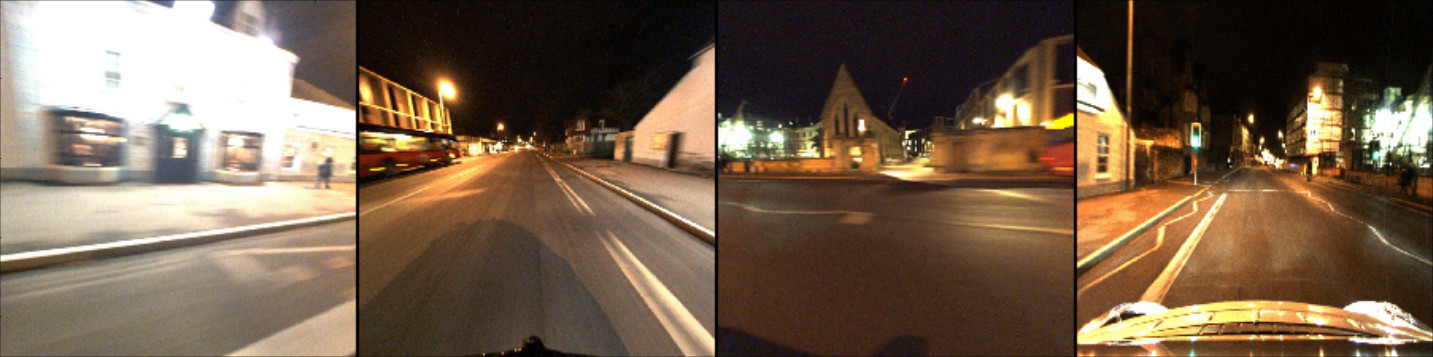
\includegraphics[width=\linewidth]{chall_loc/depth_night_im/input}		
	\end{minipage}
	
	\begin{minipage}{0.15\linewidth}
		\center\scriptsize
		Ground truth depth map
	\end{minipage}\hfill
	\begin{minipage}{0.84\linewidth}
	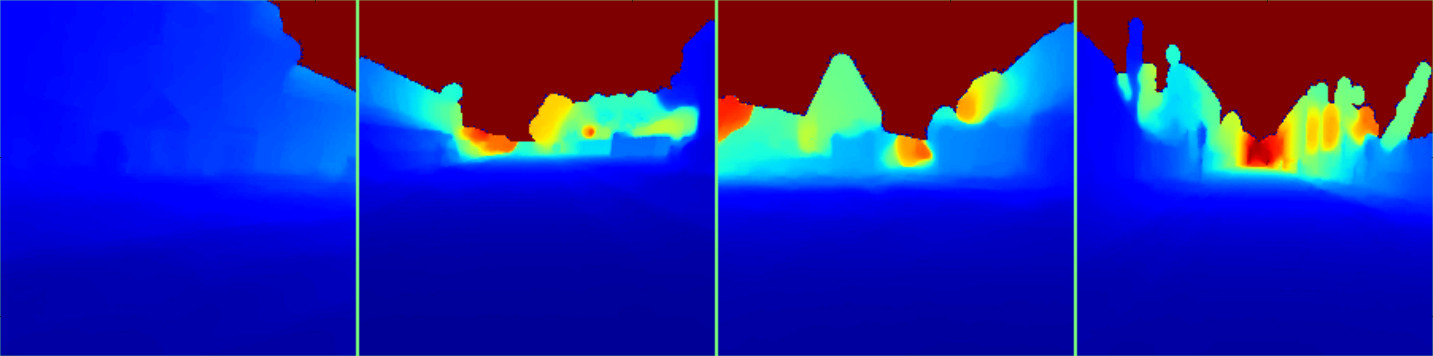
\includegraphics[width=\linewidth]{chall_loc/depth_night_im/gt}	
	\end{minipage}
	
	\begin{minipage}{0.15\linewidth}
		\center\scriptsize		
		Generated depth map after fine tuning
	\end{minipage}\hfill
	\begin{minipage}{0.84\linewidth}
	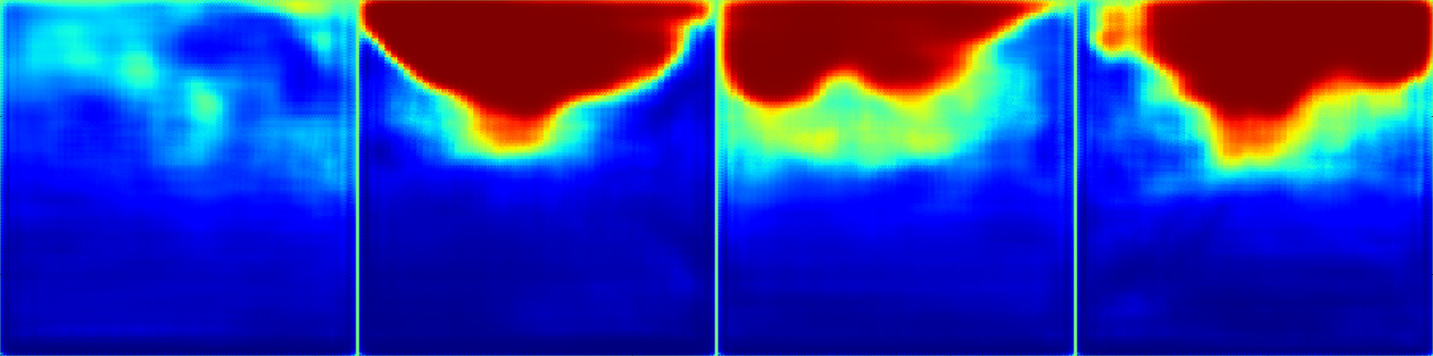
\includegraphics[width=\linewidth]{chall_loc/depth_night_im/ft}	
	\end{minipage}

	\begin{minipage}{0.15\linewidth}
		\center\scriptsize		
		Generated depth map before fine tuning
	\end{minipage}\hfill
	\begin{minipage}{0.84\linewidth}
	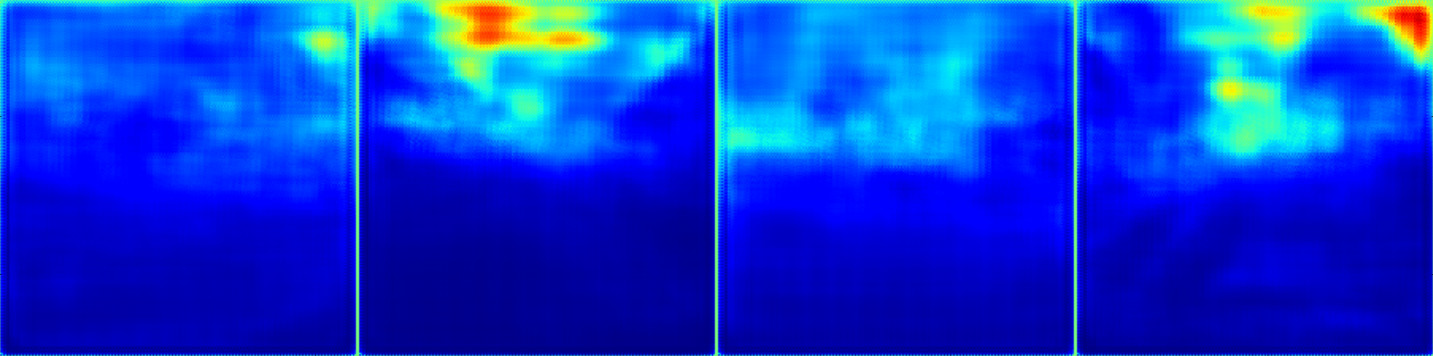
\includegraphics[width=\linewidth]{chall_loc/depth_night_im/noft}	
	\end{minipage}
	
	\caption[Effect of fine tuning with night images on decoder output]{\label{fig:mod_ex} \textbf{Effect of fine tuning with night images on decoder output:}. Decoder trained with daylight images is unable to reconstruct the scene geometry (bottom line). Fine tuning the network with less than 1000 pairs \{image, depth map\} acquired by night highly improves appearance of the generated depth maps. Maps best viewed in color.}
\end{figure}